%  LaTeX support: latex@mdpi.com 
%  In case you need support, please attach all files that are necessary for compiling as well as the log file, and specify the details of your LaTeX setup (which operating system and LaTeX version / tools you are using).

%=================================================================
\documentclass[journal,article,submit,moreauthors,pdftex]{Definitions/mdpi}
\usepackage{graphicx}
\usepackage{caption}
\usepackage{subcaption}
\graphicspath{{img/}}
\usepackage{booktabs}
\usepackage{amsmath}
\usepackage{footnote}
\usepackage{steinmetz}
%\makesavenoteenv{tabular}
%\makesavenoteenv{table}
\usepackage{fixltx2e}
\externalbibliography{yes}
\usepackage[style=numeric,backend=biber]{biblatex}
\addbibresource{Thesisref_LATEX.bib}
%\bibliography{Thesisref_LATEX.bib}
% If you would like to post an early version of this manuscript as a preprint, you may use preprint as the journal and change 'submit' to 'accept'. The document class line would be, e.g., \documentclass[preprints,article,accept,moreauthors,pdftex]{mdpi}. This is especially recommended for submission to arXiv, where line numbers should be removed before posting. For preprints.org, the editorial staff will make this change immediately prior to posting.

%--------------------
% Class Options:
%--------------------
%----------
% journal
%----------
% Choose between the following MDPI journals:
% acoustics, actuators, addictions, admsci, aerospace, agriculture, agriengineering, agronomy, algorithms, animals, antibiotics, antibodies, antioxidants, applsci, arts, asc, asi, atmosphere, atoms, axioms, batteries, bdcc, behavsci , beverages, bioengineering, biology, biomedicines, biomimetics, biomolecules, biosensors, brainsci , buildings, cancers, carbon , catalysts, cells, ceramics, challenges, chemengineering, chemistry, chemosensors, children, cleantechnol, climate, clockssleep, cmd, coatings, colloids, computation, computers, condensedmatter, cosmetics, cryptography, crystals, dairy, data, dentistry, designs , diagnostics, diseases, diversity, drones, econometrics, economies, education, ejihpe, electrochem, electronics, energies, entropy, environments, epigenomes, est, fermentation, fibers, fire, fishes, fluids, foods, forecasting, forests, fractalfract, futureinternet, futurephys, galaxies, games, gastrointestdisord, gels, genealogy, genes, geohazards, geosciences, geriatrics, hazardousmatters, healthcare, heritage, highthroughput, horticulturae, humanities, hydrology, ijerph, ijfs, ijgi, ijms, ijns, ijtpp, informatics, information, infrastructures, inorganics, insects, instruments, inventions, iot, j, jcdd, jcm, jcp, jcs, jdb, jfb, jfmk, jimaging, jintelligence, jlpea, jmmp, jmse, jnt, jof, joitmc, jpm, jrfm, jsan, land, languages, laws, life, literature, logistics, lubricants, machines, magnetochemistry, make, marinedrugs, materials, mathematics, mca, medicina, medicines, medsci, membranes, metabolites, metals, microarrays, micromachines, microorganisms, minerals, modelling, molbank, molecules, mps, mti, nanomaterials, ncrna, neuroglia, nitrogen, notspecified, nutrients, ohbm, optics, particles, pathogens, pharmaceuticals, pharmaceutics, pharmacy, philosophies, photonics, physics, plants, plasma, polymers, polysaccharides, preprints , proceedings, processes, proteomes, psych, publications, quantumrep, quaternary, qubs, reactions, recycling, religions, remotesensing, reports, resources, risks, robotics, safety, sci, scipharm, sensors, separations, sexes, signals, sinusitis, smartcities, sna, societies, socsci, soilsystems, sports, standards, stats, surfaces, surgeries, sustainability, symmetry, systems, technologies, test, toxics, toxins, tropicalmed, universe, urbansci, vaccines, vehicles, vetsci, vibration, viruses, vision, water, wem, wevj

%---------
% article
%---------
% The default type of manuscript is "article", but can be replaced by:
% abstract, addendum, article, benchmark, book, bookreview, briefreport, casereport, changes, comment, commentary, communication, conceptpaper, conferenceproceedings, correction, conferencereport, expressionofconcern, extendedabstract, meetingreport, creative, datadescriptor, discussion, editorial, essay, erratum, hypothesis, interestingimages, letter, meetingreport, newbookreceived, obituary, opinion, projectreport, reply, retraction, review, perspective, protocol, shortnote, supfile, technicalnote, viewpoint
% supfile = supplementary materials

%----------
% submit
%----------
% The class option "submit" will be changed to "accept" by the Editorial Office when the paper is accepted. This will only make changes to the frontpage (e.g., the logo of the journal will get visible), the headings, and the copyright information. Also, line numbering will be removed. Journal info and pagination for accepted papers will also be assigned by the Editorial Office.

%------------------
% moreauthors
%------------------
% If there is only one author the class option oneauthor should be used. Otherwise use the class option moreauthors.

%---------
% pdftex
%---------
% The option pdftex is for use with pdfLaTeX. If eps figures are used, remove the option pdftex and use LaTeX and dvi2pdf.

%=================================================================
\firstpage{1}
\makeatletter
\setcounter{page}{\@firstpage}
\makeatother
\pubvolume{xx}
\issuenum{1}
\articlenumber{5}
\pubyear{2019}
\copyrightyear{2019}
%\externaleditor{Academic Editor: name}
\history{Received: date; Accepted: date; Published: date}
%\updates{yes} % If there is an update available, un-comment this line

%% MDPI internal command: uncomment if new journal that already uses continuous page numbers
%\continuouspages{yes}

%------------------------------------------------------------------
% The following line should be uncommented if the LaTeX file is uploaded to arXiv.org
%\pdfoutput=1

%=================================================================
% Add packages and commands here. The following packages are loaded in our class file: fontenc, calc, indentfirst, fancyhdr, graphicx, lastpage, ifthen, lineno, float, amsmath, setspace, enumitem, mathpazo, booktabs, titlesec, etoolbox, amsthm, hyphenat, natbib, hyperref, footmisc, geometry, caption, url, mdframed, tabto, soul, multirow, microtype, tikz

%=================================================================
%% Please use the following mathematics environments: Theorem, Lemma, Corollary, Proposition, Characterization, Property, Problem, Example, ExamplesandDefinitions, Hypothesis, Remark, Definition, Notation, Assumption
%% For proofs, please use the proof environment (the amsthm package is loaded by the MDPI class).

%=================================================================
% Full title of the paper (Capitalized)
\Title{Determination of the required Power Response of Inverters to provide fast Frequency Support in Power Systems with low Synchronous Inertia}

% Author Orchid ID: enter ID or remove command
\newcommand{\orcidauthorA}{0000-0000-000-000X} % Add \orcidA{} behind the author's name
%\newcommand{\orcidauthorB}{0000-0000-000-000X} % Add \orcidB{} behind the author's name

% Authors, for the paper (add full first names)
\Author{Alejandro Rubio $^{1,\dagger,\ddagger}$\orcidA{}, Holger Behrends $^{1,\ddagger}$ and Stefan Geißendörfer $^{2,}$*}

% Authors, for metadata in PDF
\AuthorNames{Alejandro Rubio, Holger Behrends and Stefan Geißendörfer}

% Affiliations / Addresses (Add [1] after \address if there is only one affiliation.)
\address{%
$^{1}$ \quad Affiliation 1; e-mail@e-mail.com\\
$^{2}$ \quad Affiliation 2; e-mail@e-mail.com}

% Contact information of the corresponding author
\corres{Correspondence: e-mail@e-mail.com; Tel.: (optional; include country code; if there are multiple corresponding authors, add author initials) +xx-xxxx-xxx-xxxx (F.L.)}

% Current address and/or shared authorship
\firstnote{Current address: Affiliation 3}
\secondnote{These authors contributed equally to this work.}
% The commands \thirdnote{} till \eighthnote{} are available for further notes

%\simplesumm{} % Simple summary

%\conference{} % An extended version of a conference paper

% Abstract (Do not insert blank lines, i.e. \\)
\abstract{Decommissioning of conventional power plants and the installation of inverter-based renewable energy technologies decreases overall power system inertia. This reduction in system inertia has an impact in the power system frequency response when an imbalance between generation and load occurs, increasing the rate of change of frequency (RoCoF) of the system. In a future scenario where renewables are predominant in power systems and due to the natural variability of the resource, imbalances of 40\% or more are prompt to happen. When a system is islanded or operates as such and combined with low inertia, it may lead to frequency collapse. This expected high values of RoCoF shorten the response time needed before load shedding or generation curtailment take place and a subsequent possible black out occurs. Through the simulation of two scenarios with different primary reserve response, the requirements for the fleet of connected inverters was determined in terms of activation time and total power to be provided in order to avoid load shedding. This activation time was determined to be the time at which frequency would reach the load shedding value, known as critical time. With such value and knowing the time required for the synchronous reserve to deploy the imbalance power, a simple expression based on nullifying RoCoF at the critical time was obtained for the required inverter based fast power reserve. It was obtained that full activation time for inverter fast power reserve with penetration above 80\% of inverter based generation would need to be between 50-500 ms for imbalances up to 40\%; meaning that current frequency measurement techniques and renewable deployment times would not ensure system stability under the foreseen future possible power system conditions. A power ramp in the order of 300\% the load per second is necessary for fast power reserve to maintain frequency within the allowed limits.}

% Keywords
\keyword{frequency support, flexibilization, renewables, inverters}

% The fields PACS, MSC, and JEL may be left empty or commented out if not applicable
%\PACS{J0101}
%\MSC{}
%\JEL{}

%%%%%%%%%%%%%%%%%%%%%%%%%%%%%%%%%%%%%%%%%%
% Only for the journal Diversity
%\LSID{\url{http://}}

%%%%%%%%%%%%%%%%%%%%%%%%%%%%%%%%%%%%%%%%%%
% Only for the journal Applied Sciences:
%\featuredapplication{Authors are encouraged to provide a concise description of the specific application or a potential application of the work. This section is not mandatory.}
%%%%%%%%%%%%%%%%%%%%%%%%%%%%%%%%%%%%%%%%%%

%%%%%%%%%%%%%%%%%%%%%%%%%%%%%%%%%%%%%%%%%%
% Only for the journal Data:
%\dataset{DOI number or link to the deposited data set in cases where the data set is published or set to be published separately. If the data set is submitted and will be published as a supplement to this paper in the journal Data, this field will be filled by the editors of the journal. In this case, please make sure to submit the data set as a supplement when entering your manuscript into our manuscript editorial system.}

%\datasetlicense{license under which the data set is made available (CC0, CC-BY, CC-BY-SA, CC-BY-NC, etc.)}

%%%%%%%%%%%%%%%%%%%%%%%%%%%%%%%%%%%%%%%%%%
% Only for the journal Toxins
%\keycontribution{The breakthroughs or highlights of the manuscript. Authors can write one or two sentences to describe the most important part of the paper.}

%\setcounter{secnumdepth}{4}
%%%%%%%%%%%%%%%%%%%%%%%%%%%%%%%%%%%%%%%%%%
\begin{document}
%%%%%%%%%%%%%%%%%%%%%%%%%%%%%%%%%%%%%%%%%%

%%%%%%%%%%%%%%%%%%%%%%%%%%%%%%%%%%%%%%%%%%
\setcounter{section}{-1} %% Remove this when starting to work on the template.
\section{How to Use this Template}
%The template details the sections that can be used in a manuscript. Note that the order and names of article sections may differ from the requirements of the journal (e.g., the positioning of the Materials and Methods section). Please check the instructions for authors page of the journal to verify the correct order and names. For any questions, please contact the editorial office of the journal or support@mdpi.com. For LaTeX related questions please contact latex@mdpi.com.
%The order of the section titles is: Introduction, Materials and Methods, Results, Discussion, Conclusions for these journals: aerospace,algorithms,antibodies,antioxidants,atmosphere,axioms,biomedicines,carbon,crystals,designs,diagnostics,environments,fermentation,fluids,forests,fractalfract,informatics,information,inventions,jfmk,jrfm,lubricants,neonatalscreening,neuroglia,particles,pharmaceutics,polymers,processes,technologies,viruses,vision

\section{Introduction}
\label{sec:intro}
%
  As part of the international efforts set to counteract global warming, the deployment of renewable energies in the electric sector has been considered an energetic priority as a measure to reduce $CO_{2}$ emissions. This objective is also reflected in the regulatory energy policies and plans of some countries. For instance, in Germany the transformation of the electricity sector through renewables, known as ''Energiewende”, contemplates to achieve a share in electricity consumption from renewables of 80\% by 2050 [3]. As part of it, the renewable energy act, ''Erneuerbare Energien Gesetz”, regulates the expansion of renewables and convectional generation decommissioning. \\
    
 Decommissioning of convectional generating power plants and its replacement with inverter-based renewables power plants has as an effect, the reduction of system inertia and consequently increasing values of RoCoF. The relevance of system inertia is to avoid rapid changes in frequency as load-generation imbalance takes place; in this way, enough time is given to the activation of the primary power reserve to recover the balanced stable conditions[ref]. %Therefore, the need of new frequency control strategies is evident in this context. Due to the expected higher values of RoCoF, load shedding caused by low frequency and generation curtailment due to over-frequency may occur faster than nowadays grid configuration[ref]. Hence, the participation of non-synchronous generation in providing frequency support as ancillary service is a key factor in achieving high integration of renewables without jeopardizing power system reliability. \\ 
 Currently in Germany, plant commitment of renewable energy plants have a priority in the power market for dispatch due to its zero marginal cost for generation. This has an effect in market auctions and also technical implications [12]. Balancing of the residual load is provided by conventional units, so curtailment of renewable energy resources is the last prefered option for power balancing [16].\\
   
  As an immediate result of an imbalance between generation and load the system frequency starts deviating from its rated value. The range of 49.8 Hz and 50.2, in Continental Europe, should be maintained by reserves after a power imbalance. This frequency range corresponds to the ordinary operation range. The primary reserve for the interconnected system is able to withstand a power imbalance of 3 GW when the system has a total load of 150 GW [1].
  At an European level, the dimensioning reference case scenario of power loss of 3 GW has been found adequate even with high penetration of renewables [1, 16]. Nevertheless, there will be still many hours with positive residual load and due to the decommissioning of conventional power plants [16, 17]; their diminished capacity to provide balancing power services at such low inertia levels will have to be compensated by balancing services coming from renewables/storage. Additionally to the uncertainty of conventional generation availability in the German power system, is also not clear whether instantaneous reserve services from abroad would be available and if transmission capacities will be enough for such [16].\\  
 
 Some ancillary services have been included in the inverter’s capabilities; inverter based generation from PV has been employed to contribute in voltage regulation by means of providing reactive power to the grid. Similarly, other approaches have been implemented for over frequency cases, by curtailment implementation and ramping limitation of inverters when system frequency approaches an upper limit allowed by local codes [4, 5]. In the same sense, new techniques have been developed in order to enable inverter based generation, such as PV and wind, to also participate in frequency support for under-frequency cases. The most common techniques try to emulate the droop power-frequency characteristic of the synchronous machine by leaving some power headroom during normal operation, so when a system frequency sag occurs, the inverter is able to push part or the total available headroom power in order to counteract the frequency drop [6]. Hence renewable sources are not any longer operating at its maximum power point, therefore these methods also have some economic constraints. Another approach to limit the frequency drop during the seconds after an event leading to a frequency decay, is to mimic the inertial response of synchronous machines. Since PV systems do not count with rotating masses, this approach is only achievable with wind turbines and called synthetic or hidden inertia [ref]. Due to the decoupling of wind turbines from the grid dynamics, modified control strategies in the power electronics allows the controller to extract part of the stored kinetic energy in the rotating masses of the wind turbine [6]. \\
 
 Although the integration of more inverter based generations brings higher values of RoCoF, they also present the solution with the implementation of fast power reserves for frequency supports. Whereas synchronous power reserve deployment is in the order of few seconds (5-30s), power electronics implementation offer full power deployment in the order of miliseconds [ref]. Table [ref] list some important and typical time scales of the most common power electronic technologies implemented in modern power systems.
 
 Insert table with values of time from GE.
 
 

 
 
 In this investigation the conditions, which should be fulfilled by inverters in highly penetrated grids by non-synchronous generation, to provide an inverter based fast power reserve (IBFPR) are investigated. Then the required triggering time and power response to avoid under-frequency load shedding (UFLS) are estimated. Over-frequency phenomenon is treated with the same approach as the under-frequency case. The effectiveness of synthetic inertia is evaluated under some assumed future scenario conditions. Three cases are utilized in order to assess the influence of the grid size, synchronous response and common simplifications made in power system analysis. The IEEE 9 bus benchmark grid model and an electric power system in the European scale are considered for such purpose; a methodology to determine the requirements of the fleet of inverters to offer frequency support is developed. %The subsequent chapters will be covering the following content: Chapter 2 corresponds to the literature related to power system operation and primary reserve. Here an overview to the aspects behind the operation of typical power systems is presented, as well as how frequency is stablished and controlled. Additionally, the influence and contribution from inverter based generators is noted. Chapter 3 presents the methodology to estimate the power rate needed to avoid transient frequency instability. The developed method and expression for power rate are then evaluated in two cases: A micro-grid with fast primary reserve response and an electric island in a European scale with relative slow primary reserve response. A detailed demonstration of parameter setting and assumptions is presented as well. The simulation results of the implemented method in each scenario is then shown in Chapter 4; critical times, frequency nadir and power responses are obtained. A detailed discussion and analysis of the main features and trends observed in the results section, is then followed in Chapter 5. The main conclusions and areas for future work are outlined in Chapters 6 and 7 respectively.

Mention some of the results from the investigation.....
%The introduction should briefly place the study in a broad context and highlight why it is important. It should define the purpose of the work and its significance. The current state of the research field should be reviewed carefully and key publications cited. Please highlight controversial and diverging hypotheses when necessary. Finally, briefly mention the main aim of the work and highlight the principal conclusions. As far as possible, please keep the introduction comprehensible to scientists outside your particular field of research. Citing a journal paper \cite{ref-journal}. And now citing a book reference \cite{ref-book}. Please use the command \citep{ref-journal} for the following MDPI journals, which use author-date citation: Administrative Sciences, Arts, Econometrics, Economies, Genealogy, Humanities, IJFS, JRFM, Languages, Laws, Religions, Risks, Social Sciences.


%%%%%%%%%%%%%%%%%%%%%%%%%%%%%%%%%%%%%%%%%%
\section{Results}
\label{sec:results}

\subsection{Analysis of Critical Time}


When both approaches for the estimation of critical time in the IEEE model are compared, it is noticed a higher deviation between them in the low range of RoCoF. This due to the fact that in this RoCoF range
the critical time is long enough to allow the governor response of the respective synchronous generation representation. Therefore it can be stated that the simplifications in the model
have a greater influence on the results for low RoCoF and IBG penetration values; in this sense, the simplifications become less significant as the RoCoF increases in such a manner
that the activated synchronous primary reserve is not relevant in frequency support.
%Despite the discrepancy in the critical time between both approaches in the IEEE 9 bus model; the power ramp calculated for the simplified model and the extended model does
not differ from each other in a great manner as exhibit later in Figure 5 2. It is then inferred that the discrepancy in critical time estimation is compensated by the factor of
nadir time, which due to non-linearity characteristics considered in the Extended model, varies upon change in inertia and load imbalance (perturbation); contrary as the linear
simplified model in which the nadir time is invariable for perturbations.
In the theory section, the typical frequency measurement time and technologies activation time were discussed [14]. Figure 5 1 contrasts the critical times obtained from the
models with the required time for frequency measurement and full power activation from different technologies.

%insert figure here

It is observed that in the range higher than 2 Hz/s; the critical time trend for the European island and the  simplified IEEE model get closer each to other as RoCoF increases
as the extended model but for very high values. %Therefore it is inferred that under high RoCoF conditions in any of the models, the primary reserve does not significantly
counteract the frequency drop [16]. Figure 5 1 demonstrates that primary reserve can be neglected for determination of the critical time when the combination of inverter based generation and
load imbalances would lead to high values of RoCoF (>2 Hz/s); as RoCoF increases, the approximation of critical time as 1(Hz)/RoCoF narrows the difference with the results obtained from simulations [14].
 Nevertheless such simplification is applicable to the simplified IEEE model and the European island. Hence, the influence of all the dynamics and machine components, such as
generator exciter and armotisour windings, seems to improve the critical time; extending up to a 34\% the calculated time with the simplified approach. Damping torque in swing equation [7, 8] was
not considered for the IEEE simplifed model; the inclusion of such may lead to more precise times when comparing with the extended model.
%Also it is then stated the need of a fast power response to avoid frequency collapse of islanded micro-grid or an electric island in the European scale.% Even assuming that power reserve can
immediately fully activated after RoCoF reading, the 100 ms limitation is a constraint for high unbalanced islands with high penetration of IBG in the European case as
demonstrated in the result section. 

% As conclusion

%Additionally, the direct measurement of RoCoF in the 100 ms interval can lead to misleading readings [14]. In general, when penetration
%of IBG is higher than 90\%; for the 40\% imbalance an activation time between 30 and 50 ms would be needed to keep frequency within the allowed limits.
%Due to the fact that the characteristics of the interconnected scenario provided by ENTSOE were assumed to be the same than the resulting islands after a severe event; the
results for the European island can be understood as the behavior of the whole European system with bigger perturbations. The dimensioning scenario assumes a power imbalance
of 3 GW, which corresponds to a 2\% of the 150 GW load [1]. If in future a bigger dimensioning case is utilized, then synchronous response would not be enough to balance the system before load shedding occurs.

Table 5 1 exhibits the required time when the dimensioning scenario is increased up to 10\% for different IBG penetration.
IBG share (%)	Load imbalance (%)
	3	4	5	6	7	8	9	10
20	-	-	6.081	4.517	3.629	3.050	2.638	2.316
40	-	6.226	4.169	3.215	2.628	2.222	1.934	1.705
60	7.142	3.639	2.623	2.062	1.698	1.451	1.263	1.122
80	2.753	1.744	1.277	1.018	0.843	0.722	0.628	0.559
92	1.109	0.700	0.514	0.406	0.338	0.288	0.252	0.224
95	0.697	0.436	0.322	0.254	0.211	0.179	0.157	0.140
Table 5 1: Critical times for European case in seconds.



Scenarios with higher imbalance than the reference scenario combined with high penetration of DER will require fast power reserve as indicated in Table 5 1.
Nadir freq.
Nadir for 3 cases with no support: behavior of governor response
Nadir for 2 cases with synthetic inertia/critical time improvement with synthetic inertia
Nadir for 3 cases with inverter based fast power reserve


\subsection{Analysis of Synthetic Inertia and Fast Power Reserve}

\subsubsection{Effect Synthetic Inertia on Frequency}





\subsubsection{Effect of Power Ramp Response on Frequency}

When the power ramp required to meet the power load imbalance at the critical time was calculated in chapter 3; the contribution from the ramping power in diminishing system RoCoF during the inception of the perturbation until the critical time was disregarded. Therefore the fast inverter based power response values at the critical time correspond to the accelerating power at that time. Assuming an instant switching of the IBFPR at critical time, the frequency nadir would be 49 Hz (no ramping power before critical time). Nevertheless, a ramp power response was assumed instead. Therefore the calculated power ramp, when applied to the unbalanced system, commonly exhibits a frequency nadir higher than 49 Hz, due to the contribution of the ramping period. In this sense, it can be inferred that the longer the ramping period (shorter measuring time), the higher frequency nadir will be obtained. Here again the relevance of the prompt activation in time of the IBFPR. On the other hand, with the faster IBFPR activation, the ramp slope and the steady power output (Inverter based power reserve) can be diminished compromising frequency nadir.
When the activation does not takes place instantaneously, frequency nadir and therefore system stability can be compromised for some combination of system inertia and load imbalance as demonstrated in the result section. In order to assure stability a stepper ramp slope is required in order to meet the required power before critical time. That is achieved by changing equation 3-2 by the adjusted expression:
Equation 5 1
%P_IBFPR (t)=∆P*((1-t_cr⁄t_nadir ))/((t_cr-t_d ) )*t
Where td is the time delay needed to start the activation of IBFPR.
When a comparison is established beween all the calculated power ramp slopes in per unit  (pu), it is noted that with high penetration of non-synchronous power in the power system, the required power to ensure no UFLS have a consistent trend between the three models, and a close proximity in the values for RoCoF in the range of 2 to 5 Hz/s is observed between both IEEE models. Such trends can be seen in Figure 5 2.
A bigger amount of power ramp slope is needed in all the range of RoCoF for the European case. After inspecting Equation 3-2, it is noticed that the IBFPR is affected by the factor(1-t_cr⁄t_nadir ), then as nadir time increases, IBFPR increases as well. The nadir time for the European case, due to the action of the self-regulation and primary reserve deployment of 30 seconds, is in the range of 3-12 seconds (6 seconds for 80\% IBG penetration) whereas the nadir time for the simplified IEEE model is between 1-3 seconds. See Appendix III for more details in regards of nadir time.
Fast Power Reserve

So far, the power ramp required to avoid load shedding has been found for the IEEE 9 bus model with a fast governor response and for the European island with conventional primary reserve response. Hence, the investigated inverter based fast power response at critical time which remain constant afterwards, would be accounted as the fast power reserve. Similarly as primary reserve estimations are performed considering the loss of generation at certain level; for fast power reserve the results are presented for the scenarios in which imbalance could reach even 40\%.

 Figure 5 3 shows the results of the needed fast power reserve for each case under 80\% of IBG penetration. A linear behavior is exhibit by the simplified model and the European.

A proportion of almost one to one is observed for the European model, this is caused by the slow primary reserve. Therefore for imbalances higher than 3\% the fast power reserve has to cover all the imbalance. The observed offset from the one to one relation is due to the load reduction caused by the frequency drop (load self-regulation). The dashed line represents the one to one proportion. In the case of the IEEE grid; the simplified model exhibits a permanent offset from the dashed line of around 0.05 pu, this due to the action of a faster governor response. Therefore, it can be said that in such scenario, the conventional governor response of synchronous machines would cover 5\% of the imbalances starting at 8\%. Since the values for nadir time are not independent from the imbalance in the Extended model, due to the non-linearity of the model, the calculated power reserve tend to equalize the whole imbalance. As imbalance increases, the critical time decreases and the nadir time increases, this makes the reducing factor tcr/tnadir from Equation 3-2 to decrease and narrows the difference between the calculated reserve and power imbalance.
Similarly as critical time was presented in Table 5 1 the required fast power reserve in the European context is shown in Table 5 2 for extraordinary events



Table 5 2: Fast power reserve in per unit for European case
IBG share (%)	Load imbalance (%)
	3	4	5	6	7	8	9	10
20	-	-	0.025	0.038	0.049	0.060	0.070	0.081
40	-	0.016	0.030	0.041	0.052	0.063	0.073	0.083
60	0.005	0.024	0.035	0.045	0.056	0.066	0.077	0.087
80	0.016	0.028	0.039	0.049	0.062	0.070	0.080	0.09
92	0.021	0.033	0.043	0.054	0.064	0.074	0.084	0.094
95	0.024	0.035	0.045	0.055	0.065	0.075	0.085	0.096

As IBG increases the closer to the imbalance the fast power reserve needs to be. As it was demonstrated in the result section; with a faster conventional reserve, reduction in fast power reserve can be observed.
\subsection{Synchronizing effect, lack of damping torque and implications}

When the IEEE model was implemented using SIMULINK-SIMSCAPE blocks, in order to incorporate all system component dynamics; system instability was found for low inertia values in the system and due to high imbalances (with no IBFPR). In non-linear systems, the stability is not only determined by the equivalent transfer function but also it is dependent on the inputs or sources [7, 22]. In this sense the loss of stability due to huge load imbalances is explained by the non-linearity of the system. When the system is perturbed by a small change in one of the state variables in such a way that the system returns to its initial state or remains close to it; a linearization of the system can be performed and a so called small signal stability analysis can be performed [7].
In the simulations it was found how the extended model is unstable for imbalances above 15\% with a penetration of non-synchronous generation of 85\%, corresponding to a system acceleration time constant of 2.1 seconds. The diminishing of synchronous machines, and the dependency of system frequency and voltage signal from them, lead to a very weak network, where synchronizing and damping torque, which are inherent characteristics of synchronous machines are not enough to stabilize the system (assuming that such excursion of frequency and rotor speed would be allowed to happen) [7]. Although the implementation of IBFPR contributes keeping synchronous machine on step , low frequency oscillations in the rotor speed/frequency response are observed. This oscillations are created by the lack of damping torque which is provided mainly by the synchronous machines, through damping windings, field exciter and Power System Stabilizer (connected to the machines exciter). For the simplified IEEE model and the European island, only transfer functions describing an equivalent system governor were modeled. Hence in such approaches, the effect and dynamics of synchronous generator’s exciters and inter-machine interaction were not taken into account. The before mention factors influence greatly small signal stability [7, 8]
Even though the scoop of this thesis is to analyze the power-time characteristics needed to avoid frequency collapse; oscillations associated to big perturbation were observed but they could not been addressed by the simple injection of power to the system. Also in the IEEE model, when a penetration of 95\% of inverter based generation and 2\% of load imbalance are considered, UFLS is not reached but the system becomes unstable as shown in Figure 5 6 and Figure 5 5. From penetrations levels above 85\% complete frequency stability is not ensure with the injection of fast power reserve, only UFLS on the first 10 seconds approximately. Then the system becomes unstable with increasing amplitude oscillations.
It is important to note that ENTSOE in its EUROPEAN interconnected scenario, determined that there is no UFLS when an unbalance of 2\% with high contribution of non-synchronous generation occurs. Nevertheless, no inter-machine interaction was considered and therefore a similar effect as the one in Figure 5 6 could be experienced.


%%%%%%%%%%%%%%%%%%%%%%%%%%%%%%%%%%%%%%%%%%
\section{Discussion}

Authors should discuss the results and how they can be interpreted in perspective of previous studies and of the working hypotheses. The findings and their implications should be discussed in the broadest context possible. Future research directions may also be highlighted.

%%%%%%%%%%%%%%%%%%%%%%%%%%%%%%%%%%%%%%%%%%
\section{Materials and Methods}
\label{sec:method}
The transitory frequency response of the system and therefore its stable and reliable operation after a perturbation, depends on the inherent characteristics of the power system and the counteraction measurements engaged automatically by the power system. As the share of inverter based generation increases, the more sensible to instability the power system becomes. In this sense the added inverter based fast power reserve must be capable of maintaining transitory frequency value within the allowed limits. 
Two terms commonly found in the literature of power system stability will be used along this section:

\begin{itemize}[leftmargin=*,labelsep=5.8mm]
	\item \textbf{Inertia constant (H)}: It has units of seconds (s) and it is the ratio of the kinetic energy stored in the rotating masses of the generators ($E_k$ in MWs) and its nominal capacity ($S_{nom}$ in MVA).\\
	\item \textbf{Acceleration time constant (T\textsubscript{a})}: It also has the units of seconds (s) but this is the ratio of double the kinetic energy (MWs) and generators nominal power output ($P_{nom}$ in MW).\\
	 Acceleration time constant is a measure of the robustness before disturbances of the system. It could be interpreted as the required time to remove the kinetic energy from the rotating masses of the generators connected in a grid at the rate of the supplied power load. Hence, the higher the time constant, the higher the kinetic energy available. As the share of synchronous generations decreases, this constant decreases proportionally.
\end{itemize}

With $f$ as frequency, $f_0$ as nominal frequency and $\Delta P$ as power imbalance the swing equation can be expressed as follows:
%Equation 3 1
\begin{equation}
	\label{eq:swing}
	\frac{df}{dt}=\dfrac{\Delta P*f_0}{2*H*S_{nom}}=\frac{\Delta P*f_0}{T_a*P_{nom}}=\frac{\Delta P*f_0}{2*E_k}
\end{equation}
%df/dt=(∆P*f_0)/(2*H*S_nom )=(∆P*f_0)/(T_a*P_nom )=(∆P*f_0)/(2*E_k )
In this paper, the inertia constant $ H $ is used for the description of synthetic inertia in wind turbines, whereas the system acceleration constant $ T_a $ is used to express the whole system inertia related to the load in terms of real power.

\subsection{Synthetic Inertia}


Synthetic inertia is one of the new techniques that manufactures and researchers are considering to tackle with the low inertia problem in power systems  [23, 24]. Frequency support through synthetic inertia was considered with the following assumptions [6, 25]:
\begin{enumerate}[leftmargin=*,labelsep=4.9mm]
	\item Power output from synthetic inertia is limited to 10\% of wind turbine nominal power.
	\item Due to mechanical and thermal stresses, the additional power can be delivered only for a maximum time of 10 s.
	\item It is assumed that all wind turbines operate at its maximum power output. The value of 1.5 MW was selected for such purpose.
	\item In order to avoid wind turbine stall, the removed kinetic energy from the blades (injected to the grid in electrical form) it is limited to half [26].

\end{enumerate}

	An adequate control system is needed so the stored energy in the rotating blades can be extracted from the wind turbine. From the expression of power as the derivative of energy stored in the blades \eqref{eq:si}, the rate of energy extracted from the wind turbine can be obtained, considering that the rotational speed changes in time ref.

\begin{equation}
	\label{eq:si}
	P_{pu}(t)=2*H_{wt}*\omega_{pu}(t)*\dfrac{d\omega_{pu}(t)}{dt}
\end{equation}

%Equation 3 4 

Where  $H_{wt}$ is the turbine inertia constant and $\omega_{pu}$ the rotational speed in per unit.\\

\begin{figure}[h]
	\centering
	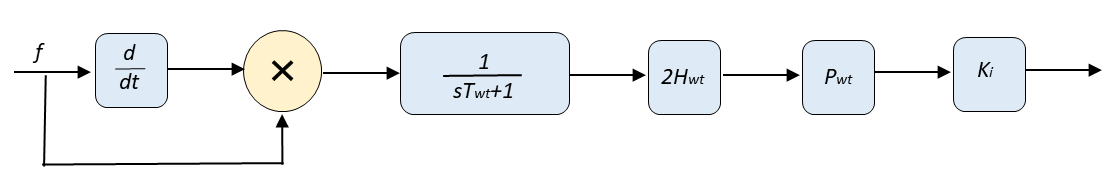
\includegraphics[width=0.6\textwidth]{/method/SI}
	\caption{Representation of equation \eqref{eq:si} in the model. In the figure it can be seen the insertion of a filter at the output of the multiplication block. A constant block $ K_i $ adjusts the initial response in the model. Since equation \eqref{eq:si} is given in pu, the output is multiplied by a constant $ P_{wt} $ representing the rated power of the turbine.}
	\label{fig:synthetic}
\end{figure}





%Equation \eqref{eq:si} was implemented in SIMULINK with the addition of a gain block $K_i$, in order to inject more power from the very beginning of the power imbalance. A filter at the signal entrance was added in order to suppress non desired oscillations on the system [24, 25].\\

%Insert diagram of synthetic inertia here

Typical values for inertia constant of wind turbines are not openly available from the manufacturers to the public. Hence an approximate value was calculated with the utilization of an equation which relates nominal power and inertia constant for wind turbines [27].
\begin{equation}
	\label{eq:wtinertia}
	H_{wt}\approx1.87*P_{nwt}^{0.0597}
\end{equation}
%Equation 3 5: Wind turbine inertia constant as function of the nominal power in MW.
%H_wt≅1.87*P_nwt^0.0597
For a wind turbine with nominal power output of 1.5 MW the value of $ H $ corresponds to 4.37 s [28].
It is assumed that all the wind turbines deliver their nominal power output. A rated rotational speed of 18 rev/min was considered [28]. To avoid the wind turbine to stall, a reduction of 5 rev/min it is allowed by the implementation of the control system. This change of rotational speed equals a change of 3 MWs reduction on kinetic energy out of a total of 6 MWs.

%Table 3 1: Constants for implementation of synthetic inertia.
\begin{table}[h]
	\caption{\label{tb:inertia}: Constants for implementation of synthetic inertia}
	\centering
	%% \tablesize{} %% You can specify the fontsize here, e.g., \tablesize{\footnotesize}. If commented out \small will be used.
	\begin{tabular}{cccc}
		\toprule
		\textbf{T\textsubscript{wt}} 	& \textbf{ H\textsubscript{wt} (s)}	& \textbf{ P\textsubscript{wt} (MW)}  & \textbf{ K\textsubscript{i}} \\
		\midrule
			1	       & 4.37		        &  1.5*$ n_{wt} $\footnote{Number of wind turbines with synthetic inertia control} & 10 \\
		%entry 2		& data			& data\\
		\bottomrule
	\end{tabular}
\end{table}

\subsection{Inverter based fast Power Reserve}


%Figure 3 1 depicts the typical frequency response when a negative power imbalance occurs in a power system. If the imbalance is high enough or the system inertia is too low, the initial RoCoF can lead to frequency %excursions below the UFLS value. The value of RoCoF is brought to zero normally by the action of the primary reserve; equalizing the power imbalance assuming no load frequency dependency. At this time the minimum value %of frequency (frequency nadir) is reached as well.
When a power system is subjected to a negative power imbalance and it is assumed that no load is rejected at UFLS frequency, this continues dropping below 49 Hz. The time at which the system frequency equals the UFLS value is then called critical time. This is the maximum available time for the inverter based reserve to deploy the required power to the system. \\

\begin{figure}[h]
	\centering
	\begin{subfigure}[h]{0.45\textwidth}
		\centering
		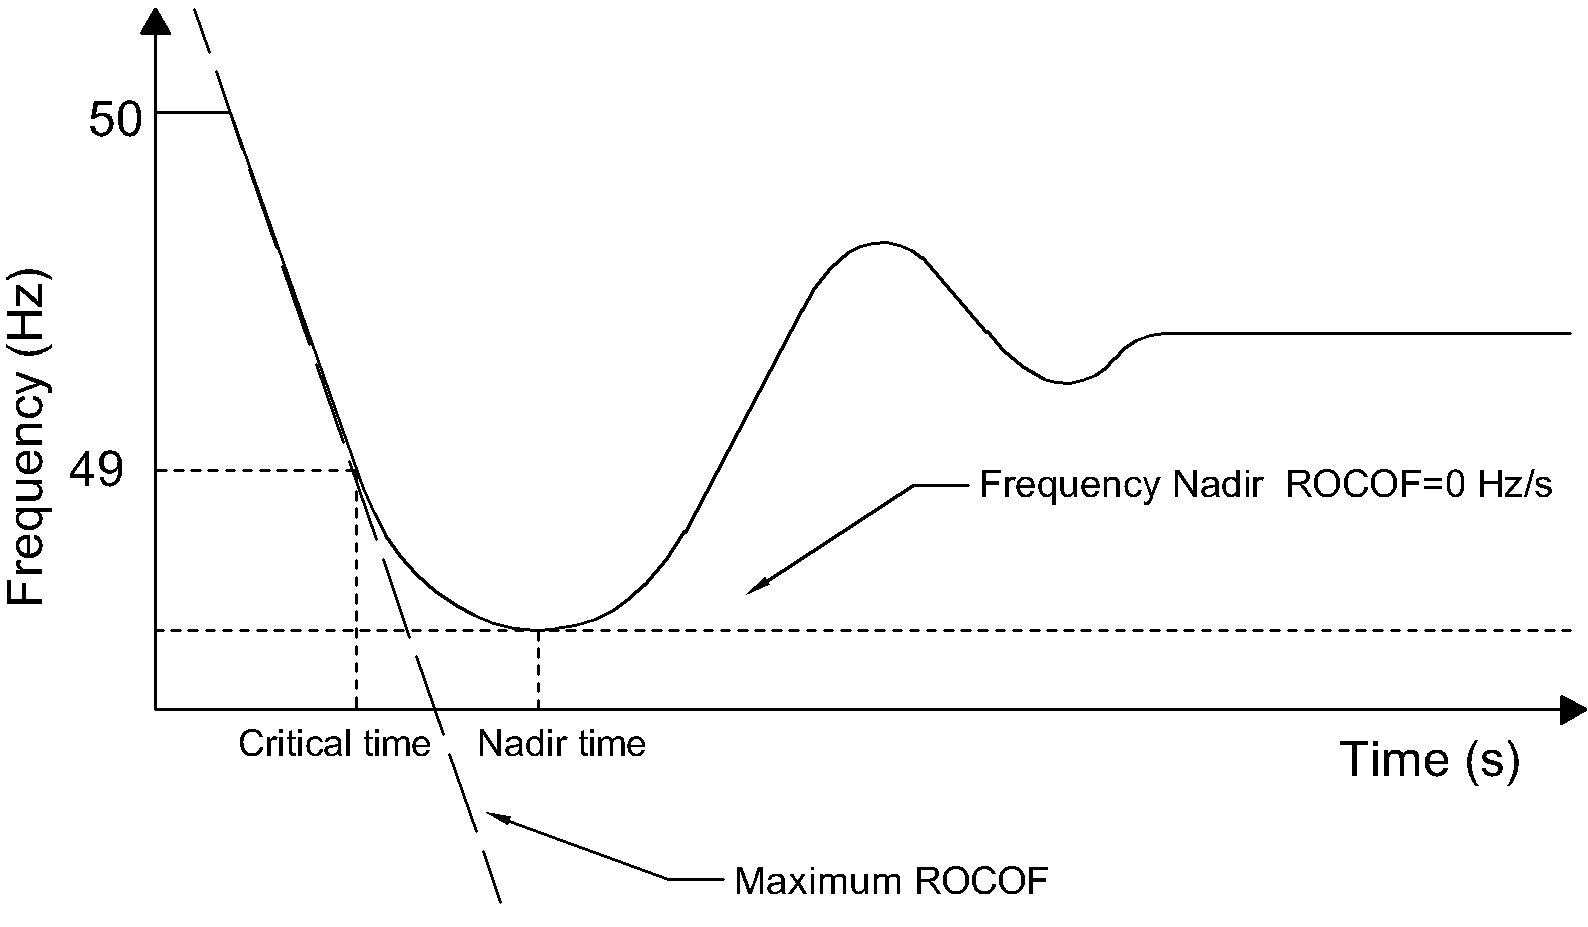
\includegraphics[width=\textwidth]{method/fig1}
		\caption{Typical frequency response leading to UFLS}
		\label{fig:freqresp_before}	
	\end{subfigure}
	\hfill
	\begin{subfigure}[h]{0.45\textwidth}
		\centering
		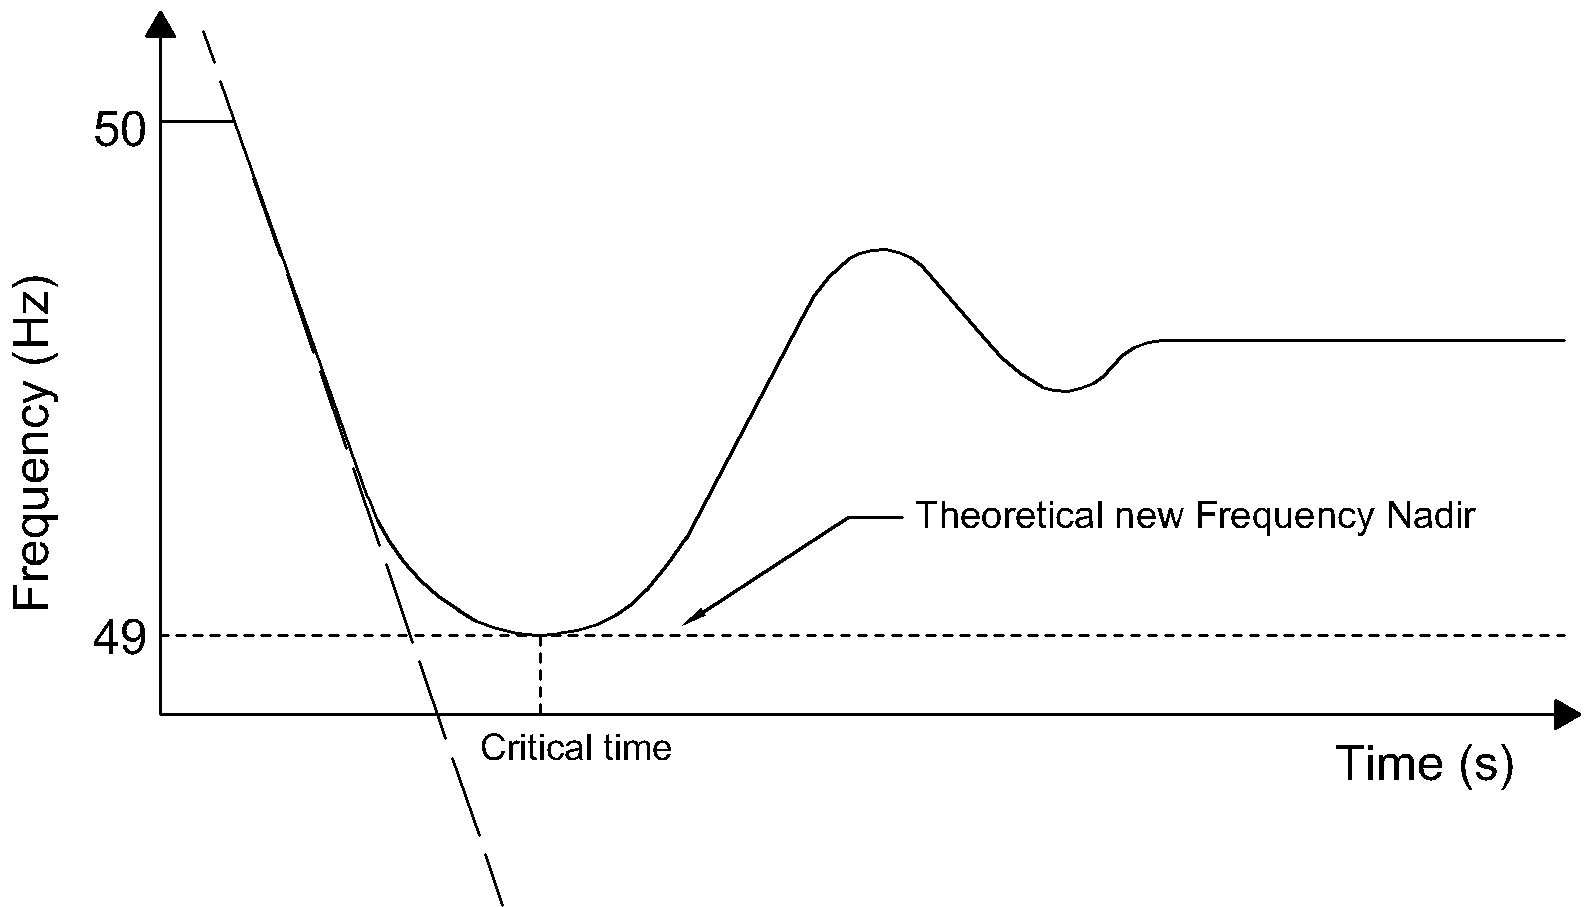
\includegraphics[width=\textwidth]{method/fig2}	
		\caption{Desired frequency response avoiding UFLS}
		\label{fig:freqresp_after}
	\end{subfigure}
	
	
	\caption{In (\textbf{a}) the frequency response goes below the 49 Hz leading to UFLS at the critical time, whereas in (\textbf{b}) the IBFPR is applied avoiding ULFS. In this case the power imbalance is compensated at the critical time by the inverters.}
\end{figure} 

In the critical condition that would lead to load shedding, it is expected from the IBFPR to at least to counteract the RoCoF at the critical time, as illustrated in Figure \ref{fig:freqresp_after}.
Recalling equation \eqref{eq:swing}; it is necessary that the machine’s accelerating power (power imbalance) become zero at the critical time.
\begin{equation}
	\label{eq:powerbalance}
	P_a (t_{cr} )=P_{mech}-P_{elec}+P_{IBFPR}=0
\end{equation} 

Where $ P_a $ is accelerating power, $ P_{mech} $ is mechanical power, $ P_{elec} $ is electrical power load, $ t_{cr} $ is the critical time and $ P_{IBFPR} $ is inverter based fast power reserve.
%Typical primary power reserve response follows the indicated behavior shown in Figure 3 . Conventional turbine governor response is frequency dependent and may not respond linearly. For the estimation of IBFPR it was %assumed a linear power deployment over time until the critical time. Inspecting Equation 3 1; it can be notice that only the power imbalance determines the rate of change in frequency in the system along with the kinetic energy stored in the rotating masses of the generators. For this reason the analysis is focused on the change on mechanical power after the event, ignoring the electrical load and mechanical power in the stable operation before the perturbation.
From the assumption of a linear mechanical power deployment is given from the synchronous machines governors, the rate of change in mechanical power, after a power imbalance $ \Delta P $, is given by $ \Delta P/t_{nadir} $, where $ t_{nadir} $ represents the time at which the frequency nadir occurs. Given the power balance at the critical time, $ t_{cr} $; the IBFPR response must be equal to $ P_{elec}-P_{mech} $, being $ P_{elec} $ equal to $ \Delta P $. %Figure 3  illustrates the behavior of both responses together. The sum of both at critical time counteracts power imbalance.


Substituting $ P_{mech} $ by $ \Delta P* t_{cr} /_{tnadir} $ and $ P_{elec} $ by $ \Delta P $ in \eqref{eq:powerbalance}, the following expression is obtained for the $ P_{IBFPR} $ at time $ t_{cr} $:
%Equation 3 2 

\begin{equation}
	\label{eq:p_at_tcr}
	P_{IBFPR} (t_{cr} )=\Delta P*(1-t_{cr}/t_{nadir} )
\end{equation}
It is assumed that $ P_{IBFPR} $ remains with a constant power output after $ t_{cr} $ long enough to stabilize the system frequency. The result of the previous equation represents the slope of the power output since the inception of the incident until the critical time, which with the implementation of IBFPR, it will be not any longer critical but rather it will be the new desired frequency nadir time.
%Equation 3 3: IBFPR before critical time.
\begin{equation}
	\label{eq:IBFPR}
	P_{IBFPR} (t)=\dfrac{\Delta P*(1-t_{cr}/t_{nadir} )*t}{t_{cr}}
\end{equation}
%P_IBFPR (t)=∆P/t_cr *(1-t_cr/t_nadir )*t

%The positive value of \eqref{eq:IBFPR} represents the injection of fast power response from renewables or storage to counteract frequency drop below of the load shedding frequency setting of 1 Hz below nominal. Nevertheless when there is an over-frequency phenomenon with surplus in generation, the negative value of \eqref{eq:IBFPR} can be taken as the power rate required to limit over-frequency to no more than 1 Hz above nominal. Similarly, critical times would apply for upper and down frequency thresholds.\\  

According to the obtained expression; it can be realized that the desired power response from the inverters depends exclusively on parameters which cannot be directly measured from the grid connection point. In a real situation the values of $\Delta P$, $ t_{nadir} $ and $ t_{cr} $ cannot be known in advance, representing this factors a challenge in the implementation of this ideal power response. Those values are dependent on the grid characteristics, the primary conventional reserve deployment time and the overall system inertia [18]. Thus two main cases are considered for the remaining analysis with the intent of covering a wider range of systems with different characteristics and dimensions.

\subsection{Simulation Cases}

As presented in the previous section, the values of critical time and frequency nadir time depend on the system imbalance and primary reserve deployment time.  In spite of assessing the influence of the grid size and the primary reserve characteristics, two main cases are considered. In both cases is assumed that the initial steady frequency is the nominal 50 Hz.


\begin{itemize}[leftmargin=*,labelsep=5.8mm]
	\item \textbf{Small scale grid case:} For the evaluation of this case typical governor data is considered in a well-known and studied benchmark grid topology as the WSCC model, also known as the IEEE 9 bus model. Synchronous reserve deployment is in the order of a few seconds due to governor response [7, 11].
	\subitem Scenario A - Simplified Model: The power system is represented by an equivalent single machine model in which losses are neglected. It is investigated the critical time for inverters' activation and the required IBFPR is  also determined. Furthermore, the impact of synthetic inertia and the frequency measurement delay in frequency response is analyzed.
	\subitem Scenario B - Extended Model: All the power system components (transmission lines, transformers, exciters and governors of the three generators) and its dynamic characteristics are considered in the IEEE 9 bus model.\\
	\item \textbf{Large scale grid case:} The European grid scale in which all the synchronous machines are modeled and simplified as one single machine, provided with the characteristic expected from the overall system. Synchronous primary reserve deployment is in the order of $ \sim30 $ s [1, 19]. Island frequency response is assumed to be the same that the European response analyzed by ENTSOE ref.
\end{itemize}



\subsection{Simplified IEEE 9 bus Model}
\label{ssec:simpleieee}
%Microgrids can operate connected to the bulk transmission/distribution system or stand alone. In any case
%It is assumed that imbalances could occur due to internal faults when island configuration is considered or islanding from the external system results from a contigency while a considerable amount of power load of the microgrid was being `imported’ or `exported’. For the study of power systems and the increasing interest in stability analysis for DER integration, the IEEE benchmarks represent a widely used option, based on some real data. This is also the case of the IEEE 9 bus model or WSCC (Western System Coordinated Council). The IEEE 9 bus model is a representation of the former western interconnected power system of North America of 1967. For stability and reliability studies, this system has been employed in many publications as study case [20], which allows the comparison of results. Figure 3 3 illustrates grid’s configuration. 
As a first step to evaluate the impact of inverter based generation and power imbalances in the grid, the whole system is simplified as one single generating unit; neglecting all losses in the system (Transformers, transmission lines and generators) with the assumption that the mechanical output of the prime mover is the same than the electrical power output at generator terminals. Table \ref{tb:gridelements} provides a summary of the elements comprising the base model.\\

\begin{table}[h]
	\caption{\label{tb:gridelements}:Elements of the IEEE 9 bus model.}
	\centering
	%% \tablesize{} %% You can specify the fontsize here, e.g., \tablesize{\footnotesize}. If commented out \small will be used.
	\begin{tabular}{ccc}
		\toprule
		\textbf{}	& \textbf{Quantity}\\
		\midrule
		Buses		& 9			\\
		Transformers		& 3			\\
 		Transmission Lines			& 6 \\
		Generators			& 3 \\
 		Load			&  315 MW  \\
		\bottomrule
	\end{tabular}
\end{table}





Figure \ref{fig:ieeesimple} is the block representation of the swing equation \eqref{eq:swing}, it only differs in the fact that blocks representing the inverter based generation have been included. The mechanical power is represented by the output of a steam turbine governor model, which is used to represent the synchronous machine [8]. When equilibrium is lost, the accelerating power is multiply by the transfer function $ 1/(2*H*S) $, where $ H $ is the machine’s inertia constant and $ S $ is the machine’s power rating. From \eqref{eq:swing} this product equals the derivative of frequency, therefore an integrator block is added to obtain the frequency response [7, 21, 22]. A feedback loop is added and an error signal obtained from the reference frequency so the synchronous machine can react as frequency deviates from nominal. \\ 

\begin{figure}[h]
	\centering
	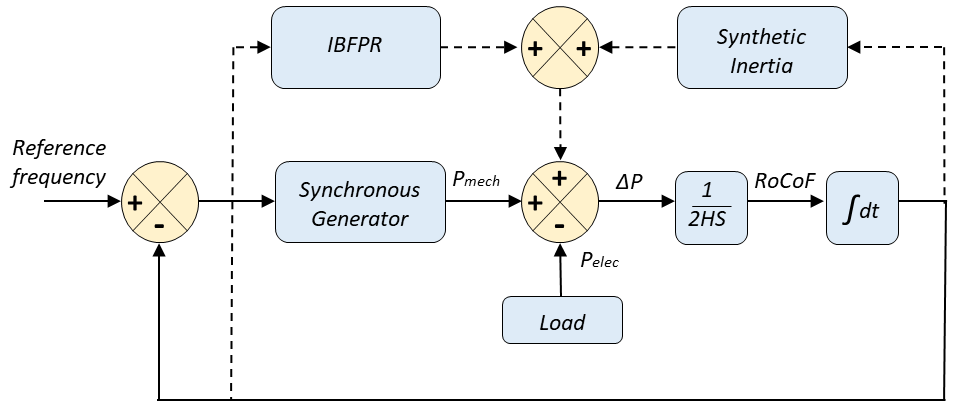
\includegraphics[width=0.6\textwidth]{/method/ieee}
	\caption{Simplified representation of the IEEE 9 bus model. Blocks linked by the solid line represent the conventional swing equation given by \eqref{eq:swing}. Represented with doted lines, the respective frequency signals to the blocks of IBFPR and synthetic inertia, which add power to the system.}
	\label{fig:ieeesimple}
\end{figure}


The values of kinetic energy and time constants of a synchronous machines of 835 MVA were selected to represent the synchronous response, with the load of 315 MW the system acceleration time constant is 14 s [8], which is approximately today’s Europe acceleration constant [1]. This is the base scenario where an 100\% synchronous generation is assumed . For the sake of evaluating the impact of the penetration of inverter based generation; the values of lower capacity generators were selected, diminishing in the sense the total system inertia [8].\\% assuming the compensation of the remaining power by a constant power source representing the inverter based generation, decreasing in this manner the total system acceleration time constant, thus the kinetic energy of the generator. Up to this point, neither synthetic inertia nor frequency support from renewables is considered. Inverter based power output remains constant before, during and after the perturbation. Therefore the system imbalance is covered only by the synchronous equivalent machine.





Even though load imbalances up to 40\% were simulated in each inertia scenario, for estimation of the critical time the power capacity limit of the generators was disregarded. The negative imbalance was simulated by increasing the system load. A block diagram representing the system shown in Figure \ref{fig:ieeesimple} was implemented in SIMULINK with different combinations of power imbalance and system inertia. %With the help of a MATLAB code several simulations were run and the critical and nadir times acquired for each scenario. With the calculated times, the IBFPR to avoid load shedding under each scenario was calculated as given by Equation 3 3 and it is shown in the Results section.
%All the acquired values of critical time, as result from the simulations, are then related with the system RoCoF, so a regression can be performed and link the critical time with system RoCoF.
%For the conditions of the system and the employment of the fitting tool provided by MATLAB, an expression is obtained for critical time as a function of RoCoF.
%For unstable conditions the maximum critical time is 2.7 seconds. Therefore critical time must be lower or equal to that value; calculating in this way that the minimum RoCoF for activation as 0.6143 Hz/s, when the fitting equation obtained from the regression is used.

\subsection{Extended IEEE 9 bus Model}

%It was previously stated that in the first approach, only the total load was considered in the simulations as well as the synchronous generation represented by one single machine and no system losses. 
Since it is desired to compare the results obtained in \ref{ssec:simpleieee} against some model that takes into account the whole system components, losses and dynamics; An  extended representation of the IEEE 9 bus model was implemented in SIMULINK [20]. In this representation, simulations for different values of system inertia and load imbalance were performed, similarly as it was done with the simplified representation of the model. Figure \ref{fig:ieeeext} shows the extended IEEE 9 bus grid architecture with IBG added.\\
\begin{figure}[h]
	\centering
	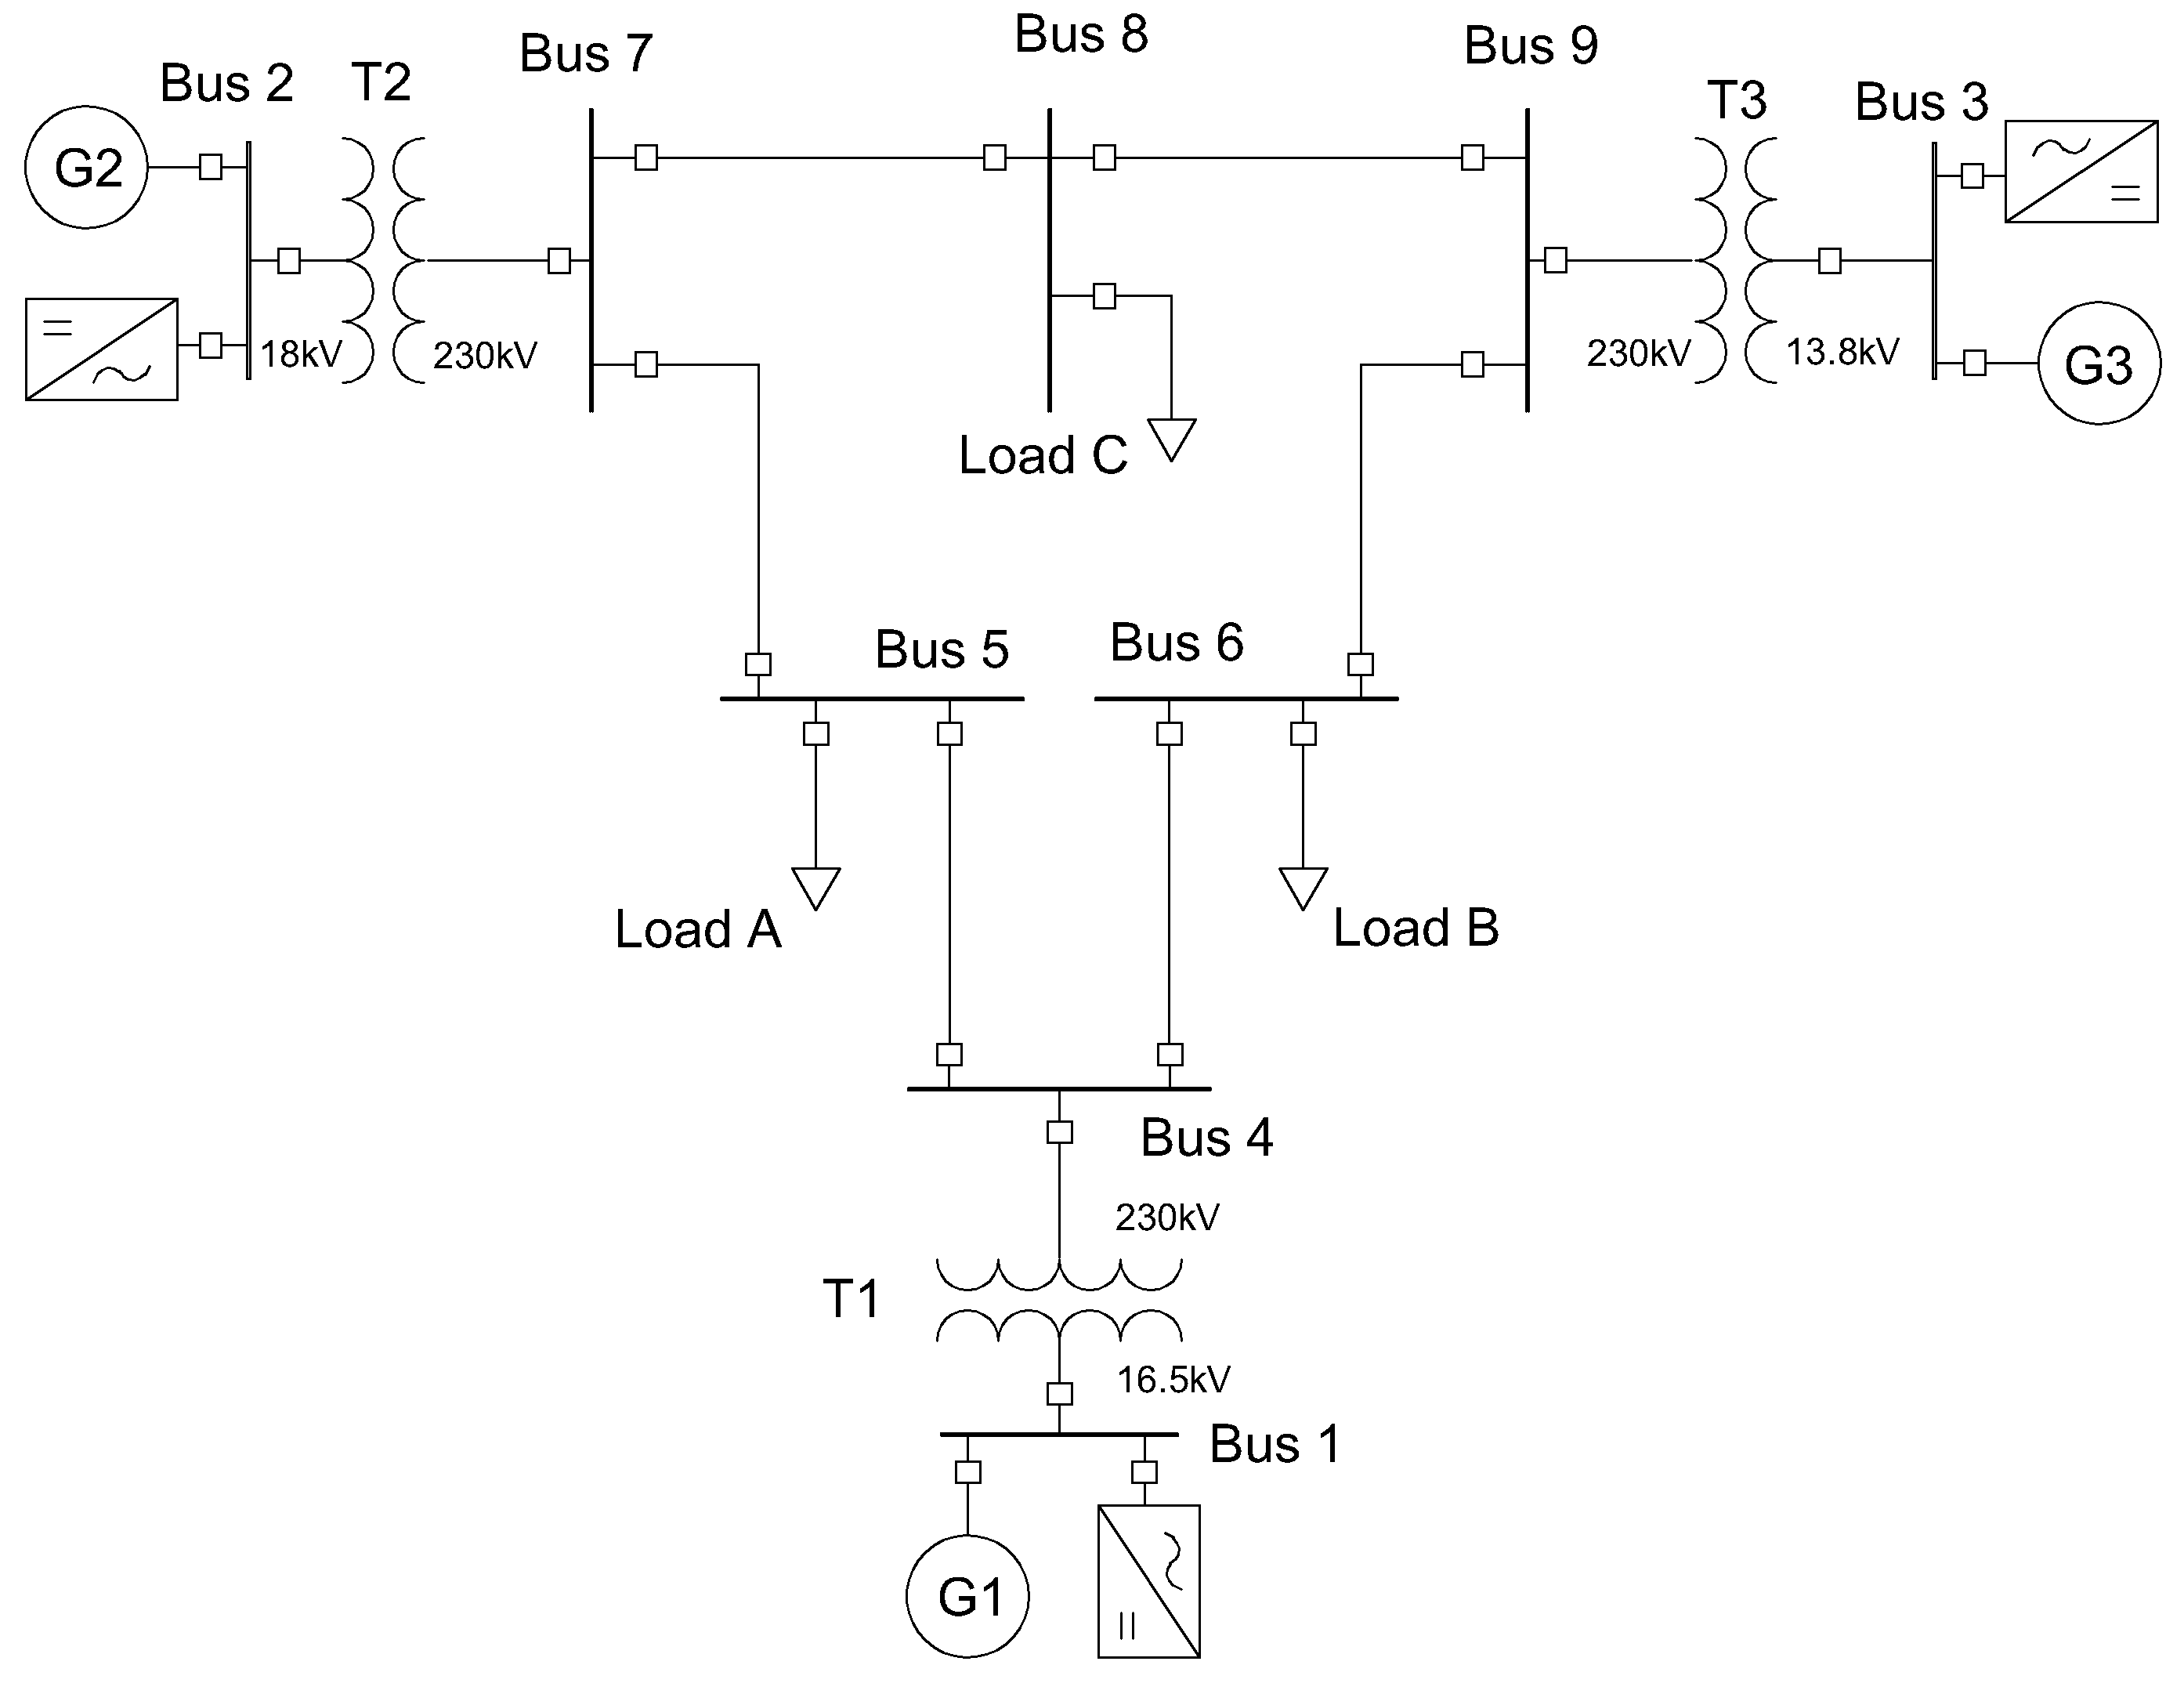
\includegraphics[width=0.5\textwidth]{/method/IEEE_FPRmodel}
	\caption{One line diagram of the IEEE 9 bus model. The inverter based frequency response has been added At the same bus of the generating units.}
	\label{fig:ieeeext}
\end{figure}
In order to evaluate the validity of the equation describing the IBFPR needed to avoid ULFS, the IEEE model was modified with the insertion of ideal controlled power sources blocks, which were set up to inject power into the grid accordingly to the simulated scenario. Therefore, no means of frequency measurement were included and only IBFPR was assessed.
Similarly as it was done in section \ref{ssec:simpleieee}, the total acceleration time constant of the system equals 14 s. Hence the same kinetic energy should be distributed among the three generators' rotating masses in the extended model as in the simplified representation. From \eqref{eq:t_sys} it can be easily calculated that the system kinetic energy with 14 s is 2205 MWs (100\% synchronous generation).
\begin{equation}
	\label{eq:t_sys}
	T_{sys}=(2*E_{k})/P_{load}
\end{equation}
 
Due to the fact that inverter based generation reduces the system kinetic energy; for different levels of inverter based generation,  the generators nominal capacity values were kept constant and the inertia constant of each machine multiplied by the synchronous share factor $ fss $. The total kinetic energy of the system is the summation of all units. In such manner the synchronous generators in the initial state of equilibrium represent both power sources, inverter based plus synchronous.\\
%Equation 3 7
%E_k=2*(H*f_ss)*S
In order to start the simulations in steady state, a load flow calculation of the grid was carried out with the objective of calculating the initial conditions for the exciter and prime mover models. 
Table\ref{tb:initial} summarizes the main values for setting system initial conditions; acquired from the power flow tool provided by SIMSCAPE.


\begin{table}[h]
	\caption{\label{tb:initial}: Steady state initial conditions of the system}
	\centering
	%% \tablesize{} %% You can specify the fontsize here, e.g., \tablesize{\footnotesize}. If commented out \small will be used.
	\begin{tabular}{ccccc}
		\toprule
		\textbf{Bus number}	& \textbf{Bus Type}	& \textbf{Voltage (pu)}& \textbf{Active Power (MW)}& \textbf{Reactive Power (MVAr)}\\
		\midrule
		1		& Slack			& 1.04 $\phase{0^{\circ}} $     &    72.2    & 25.64    \\
		2		& PV			& 1.025 $\phase{9.83^{\circ}} $      & 163      & 8     \\
		3		& PV			& 1.025 $\phase{4.63^{\circ}} $     & 85       &    -9.41 \\
		5		& PQ			& 0.9949 $\phase{-4.42^{\circ}} $       &125       &  50    \\
		6		& PQ			& 1.01211 $\phase{-4.16^{\circ}} $      &   90     &  30   \\
		8		& PQ			& 1.0172 $ \phase{0.17^{\circ}} $       &  100     &   35   \\
		
		\bottomrule
	\end{tabular}
\end{table}


\subsubsection{IBFPR Representation}


The IBFPR was modeled as controlled current sources. These controlled sources inject active power according to the load imbalance and system inertia simulated. The continuous measurement of voltage is required in order to determine the amount of current needed to supply the requested power. The IBFPR will have symmetrical and balanced characteristics. Due to this reason, the magnitude and angle of the current phasor will be obtained from the positive sequence of the measured voltage. From the definition of complex power and voltage symmetrical components in three phase systems \eqref{eq:complex_p}, the positive sequence component of phase voltage and line current are obtained. [21] 

\begin{equation}
\label{eq:complex_p}
S_{3\varphi}^1=3*V_{LN}^1*\bar{I_{L}}^1
\end{equation}

This equation is valid for RMS values of voltage and current; nevertheless the measured voltage values and the sought current values are given in peak values, the equation for power and current become:

\begin{equation}
\label{eq:power_seq}
S_{3\varphi}^1=\dfrac{3*V_{LNpeak}^1*\bar{I_{Lpeak}}^1}{2}
\end{equation}

%In the SIMULINK model the voltage measurement probes are connected at the medium voltage side of the transformes. %Figure 3 12 shows the block diagram implemented to obtain the positive symmetrical component of line voltage and the positive sequence of current that will be provided by the subsystem to meet to needed power from the ramp input depending on the voltage readings. :

 

\begin{equation}
\label{eq:current_seq}
I_{Lpeak}^1=\dfrac{\bar{2*S_{3\varphi}^1}}{3*V_{LNpeak}^1}
\end{equation}
%Equation 3 10
%〖I_Lpeak〗^1=¯(((2*〖S_3ⱷ〗^1)/(3*〖V_LNpeak〗^1 )))
With the help of the \textbf{a} operator ($-0.5+j\sqrt{3}$ or $ 1\phase{120^{\circ}}) $ the values of the positive sequence component of phase voltage can be obtained. \\
From $ V_a +V_b+V_c=0$ and $ V_a^1=\frac{V_a+ aV_b+a^2 V_c}{3} $:
\begin{align*}
	 V_a^1 & =\dfrac{V_a+ aV_b-a^2 V_b-a^2}{3} \\
	& =\dfrac{V_a*(1-a^2)+ aV_b*(1-a)}{3} 
\end{align*}

Since $V_{an}^1=\frac{V_a^1}{\sqrt{3}\phase{30^{\circ}}}$, $\sqrt{3}\phase{30^{\circ}}=1-a^2 $ and $ \sqrt{3}\phase{-30^{\circ}}=1-a $ then after some algebraic manipulation the expression for $ V_{an}^1 $ becomes:

\begin{equation}
	\label{eq:volt_seq}
	V_{an}^1=\dfrac{V_a-a^2 V_b}{3}
\end{equation}

With the obtained expressions  for the positive sequence of phase voltage \eqref{eq:volt_seq} and complex power \eqref{eq:power_seq}, the needed current \eqref{eq:current_seq} to supply the IBFPR related to the measured voltages can be implemented in SIMULINK as depicted in FIGUREXXX. The ramping function will last until the critical time is reached, afterwards, the IBFPR output will remain constant.

\subsection{Large Scale Case: Europe Power System}

Under normal operation ENTSOE has reported values of RoCoF in the range of 5-10 mHz/s for power outages of 1 GW in the current interconnected power system. If an imbalance event of more than 3 GW occurs with depleted primary reserve, extraordinary values of frequency and RoCoF might be reached. After serious disturbances the Continental European Power System has experienced RoCoF between 100 mHz/s and 1 Hz/s. Imbalances of 20\% or more along with RoCoF greater than 1 Hz/s have been determined by experience to be critical [1].
ENTSOE has determined that under the case of the reference scenario (The loss of 3 GW generation with 150 GW load and 2\%/Hz self-regulation) in the interconnected operation, the influence of inverter based generation, and therefore the reduction of system inertia would not jeopardize system stability. Due to the expected increase of non-synchronous generation in the future, international power trade and renewables variability; ENTSOE estates in its future split reference scenario that the power system must be capable of withstanding imbalances greater than 40\% with RoCoF of 2 Hz/s or higher. Under these circumstances the resulting islands must avoid load shedding. Hence, only the split scenario is considered for further analysis.

When considering the system blackout of November 4th 2006, in which four electric islands resulted from the European system split; system blackout due to under frequency was experienced in the so known western area. This island, at the moment of split, had approximately a load of 190 GW (27\% more than the low load scenarioENTSOE ) [29]. For its comparable `size’ and the uncertainty of knowing beforehand the resulting islands after a major contingency, the selected load for simulation was the same as the ENTSOE reference scenario as well as the primary reserve deployment time. To simulate the behavior of the resulting island in the European split scenario; a simplified approach was selected. Similarly as it was done with the simplified block model for the IEEE 9 bus model, in the equivalent European representation all the synchronous generation will be represented by a single machine, which will provide governor response when a perturbation takes place. Additional to the synchronous response, a load response of 2\% was added to the model, which means that for every Hertz reduced or augmented, the load will reduce or increase by a 2\% [1]. \\
 
%Figure 3 15 depicts the results of ENTSOE for the interconnected reference scenario frequency response model. It is intended that the implemented model for the island would perform in a similar way like the ENTSOE model for the same conditions [1].
In order to fit the behavior of the system to the modeled by ENTSOE, an additional block was added the IEEE simplified model in the steam turbine governor; this was done with the intention of adjusting the time response of the primary reserve as much as possible to the desired one. With this approach, the primary power reserve can be easily tuned with the assistance of the Control System Tuner App available in MATLAB. The period of time of utmost interest for analysis is from the inception of the power imbalance and the nadir time. Therefore, the system must perform as similar as possible in this region compared to the ENTSOE reference, whereas after the nadir time, the disparity between responses can be neglected. In the European scale the reserves must be completely deployed within 30 s after the occurrence of the disturbance.  






\subsubsection{System Parameters}

A power system of $ n $ number of synchronous machines is assumed; having each of them a capacity $ S $ in MVA, a nominal power $ P_{nom} $ in MW.
Assuming that each machine operates at a de-load factor $ dl $ of $ P_{nom} $; with an acceleration constant equal to $ T_{nom} $ then the number of machines $ n $, for the load $ P_{syncload} $, served by synchronous machines is:
%Equation 3 12
%n=P_(load_sync)/(P_nom*dl)
\begin{equation}
	n=\dfrac{P_{syncload}}{P_{nom}*dl}
\end{equation}
Then the time acceleration constant of the system $ T_{sys} $ can be obtained as follows:
\begin{align}
	T_{sys} &=\dfrac{\sum_{i=1}^nP_i*T_i}{P_{LOAD}}\nonumber  \\ 
	 &=\dfrac{nP_{nom}*T_i}{P_{LOAD}}\nonumber \\
	&=\dfrac{P_{syncload}*T_{nom}}{P_{LOAD}*dl}\nonumber\\	
		&=\dfrac{Sync share*T_{nom}}{dl} \label{eq:tsyseuro}
\end{align}




In this sense the system time acceleration constant can be calculated with a synchronous share of 100\%, resulting in $ T_{sys}=12.5 $ s  with values of $ T_{nom}=10 $ s [1, 8], and a de-load factor $ dl=0.8 $.
The values of the additional block in the model are set in order to have a step response with 2\% overshoot and a time constant of 8 seconds [22].
Considering only the swing equation, as done in the model, it can be demonstrated that the RoCoF and therefore the frequency response of the system is only dependent on the percentage of load imbalance and the system acceleration time constant.
From the definition of RoCoF as $ \frac{df}{dt}=\frac{\Delta P*f_0}{2*E_k} $ and  $ T_{sys}=\frac{2*E_k}{P_{LOAD}} $ :

\begin{align}
	\dfrac{df}{dt} &=\dfrac{\Delta P*f_0}{P_{LOAD}*T_{sys}} \nonumber\\
	&=\dfrac{\Delta P_{pu}*f_0}{P_{LOAD}*T_{sys}}
	\label{eq:dfdpeuro}
\end{align}
In \eqref{eq:dfdpeuro} the value of $ \Delta P_{pu} $ is the normalized value of power imbalance having as base power the value of load $ P_{LOAD} $. As shown in the equation, when only the swing equation is considered, the frequency response is only dependent on system acceleration constant and the relative value of imbalance. This relative value of imbalance varies during time, depending on load response to change on frequency and the response of primary reserve of the system.



%Materials and Methods should be described with sufficient details to allow others to replicate and build on published results. Please note that publication of your manuscript implicates that you must make all materials, data, computer code, and protocols associated with the publication available to readers. Please disclose at the submission stage any restrictions on the availability of materials or information. New methods and protocols should be described in detail while well-established methods can be briefly described and appropriately cited.

%Research manuscripts reporting large datasets that are deposited in a publicly available database should specify where the data have been deposited and provide the relevant accession numbers. If the accession numbers have not yet been obtained at the time of submission, please state that they will be provided during review. They must be provided prior to publication.

%Interventionary studies involving animals or humans, and other studies require ethical approval must list the authority that provided approval and the corresponding ethical approval code.

%%%%%%%%%%%%%%%%%%%%%%%%%%%%%%%%%%%%%%%%%%
\section{Conclusions}

This section is not mandatory, but can be added to the manuscript if the discussion is unusually long or complex.

%%%%%%%%%%%%%%%%%%%%%%%%%%%%%%%%%%%%%%%%%%
\section{Patents}
This section is not mandatory, but may be added if there are patents resulting from the work reported in this manuscript.

%%%%%%%%%%%%%%%%%%%%%%%%%%%%%%%%%%%%%%%%%%
\vspace{6pt}

%%%%%%%%%%%%%%%%%%%%%%%%%%%%%%%%%%%%%%%%%%
%% optional
%\supplementary{The following are available online at \linksupplementary{s1}, Figure S1: title, Table S1: title, Video S1: title.}

% Only for the journal Methods and Protocols:
% If you wish to submit a video article, please do so with any other supplementary material.
% \supplementary{The following are available at \linksupplementary{s1}, Figure S1: title, Table S1: title, Video S1: title. A supporting video article is available at doi: link.}

%%%%%%%%%%%%%%%%%%%%%%%%%%%%%%%%%%%%%%%%%%
\authorcontributions{For research articles with several authors, a short paragraph specifying their individual contributions must be provided. The following statements should be used ``conceptualization, X.X. and Y.Y.; methodology, X.X.; software, X.X.; validation, X.X., Y.Y. and Z.Z.; formal analysis, X.X.; investigation, X.X.; resources, X.X.; data curation, X.X.; writing--original draft preparation, X.X.; writing--review and editing, X.X.; visualization, X.X.; supervision, X.X.; project administration, X.X.; funding acquisition, Y.Y.'', please turn to the  \href{http://img.mdpi.org/data/contributor-role-instruction.pdf}{CRediT taxonomy} for the term explanation. Authorship must be limited to those who have contributed substantially to the work reported.}

%%%%%%%%%%%%%%%%%%%%%%%%%%%%%%%%%%%%%%%%%%
\funding{Please add: ``This research received no external funding'' or ``This research was funded by NAME OF FUNDER grant number XXX.'' and  and ``The APC was funded by XXX''. Check carefully that the details given are accurate and use the standard spelling of funding agency names at \url{https://search.crossref.org/funding}, any errors may affect your future funding.}

%%%%%%%%%%%%%%%%%%%%%%%%%%%%%%%%%%%%%%%%%%
\acknowledgments{In this section you can acknowledge any support given which is not covered by the author contribution or funding sections. This may include administrative and technical support, or donations in kind (e.g., materials used for experiments).}

%%%%%%%%%%%%%%%%%%%%%%%%%%%%%%%%%%%%%%%%%%
\conflictsofinterest{Declare conflicts of interest or state ``The authors declare no conflict of interest.'' Authors must identify and declare any personal circumstances or interest that may be perceived as inappropriately influencing the representation or interpretation of reported research results. Any role of the funders in the design of the study; in the collection, analyses or interpretation of data; in the writing of the manuscript, or in the decision to publish the results must be declared in this section. If there is no role, please state ``The funders had no role in the design of the study; in the collection, analyses, or interpretation of data; in the writing of the manuscript, or in the decision to publish the results''.}

%%%%%%%%%%%%%%%%%%%%%%%%%%%%%%%%%%%%%%%%%%
%% optional
\abbreviations{The following abbreviations are used in this manuscript:\\

\noindent
\begin{tabular}{@{}ll}
MDPI & Multidisciplinary Digital Publishing Institute\\
DOAJ & Directory of open access journals\\
TLA & Three letter acronym\\
LD & linear dichroism
\end{tabular}}

%%%%%%%%%%%%%%%%%%%%%%%%%%%%%%%%%%%%%%%%%%
%% optional
\appendixtitles{no} %Leave argument "no" if all appendix headings stay EMPTY (then no dot is printed after "Appendix A"). If the appendix sections contain a heading then change the argument to "yes".
\appendix
\section{}
\unskip
\subsection{}
The appendix is an optional section that can contain details and data supplemental to the main text. For example, explanations of experimental details that would disrupt the flow of the main text, but nonetheless remain crucial to understanding and reproducing the research shown; figures of replicates for experiments of which representative data is shown in the main text can be added here if brief, or as Supplementary data. Mathematical proofs of results not central to the paper can be added as an appendix.

\section{}
All appendix sections must be cited in the main text. In the appendixes, Figures, Tables, etc. should be labeled starting with `A', e.g., Figure A1, Figure A2, etc.

%%%%%%%%%%%%%%%%%%%%%%%%%%%%%%%%%%%%%%%%%%
\reftitle{References}

% Please provide either the correct journal abbreviation (e.g. according to the “List of Title Word Abbreviations” http://www.issn.org/services/online-services/access-to-the-ltwa/) or the full name of the journal.
% Citations and References in Supplementary files are permitted provided that they also appear in the reference list here.

%=====================================
% References, variant A: external bibliography
%=====================================
\printbibliography

%\bibliography{Thesisref_LATEX.bib}

%=====================================
% References, variant B: internal bibliography
%=====================================
%\begin{thebibliography}{999}
% Reference 1
%\bibitem[Author1(year)]{ref-journal}
%Author1, T. The title of the cited article. {\em Journal Abbreviation} {\bf 2008}, {\em 10}, 142--149.
% Reference 2
%\bibitem[Author2(year)]{ref-book}
%Author2, L. The title of the cited contribution. In {\em The Book Title}; Editor1, F., Editor2, A., Eds.; Publishing House: City, Country, 2007; pp. 32--58.
%\end{thebibliography}
%\printbibliography
% The following MDPI journals use author-date citation: Arts, Econometrics, Economies, Genealogy, Humanities, IJFS, JRFM, Laws, Religions, Risks, Social Sciences. For those journals, please follow the formatting guidelines on http://www.mdpi.com/authors/references
% To cite two works by the same author: \citeauthor{ref-journal-1a} (\citeyear{ref-journal-1a}, \citeyear{ref-journal-1b}). This produces: Whittaker (1967, 1975)
% To cite two works by the same author with specific pages: \citeauthor{ref-journal-3a} (\citeyear{ref-journal-3a}, p. 328; \citeyear{ref-journal-3b}, p.475). This produces: Wong (1999, p. 328; 2000, p. 475)


%%%%%%%%%%%%%%%%%%%%%%%%%%%%%%%%%%%%%%%%%%
%% optional
\sampleavailability{Samples of the compounds ...... are available from the authors.}

%% for journal Sci
%\reviewreports{\\
%Reviewer 1 comments and authors’ response\\
%Reviewer 2 comments and authors’ response\\
%Reviewer 3 comments and authors’ response
%}

%%%%%%%%%%%%%%%%%%%%%%%%%%%%%%%%%%%%%%%%%%
\end{document}
